% !TeX root = ../main.tex

\tikzset{%
  every neuron/.style={
    circle,
    draw,
    minimum size=1cm
  },
  neuron missing/.style={
    draw=none, 
    scale=3,
    text height=0.3cm,
    execute at begin node=\color{black}$\vdots$
  },
}

\vspace{.6cm}

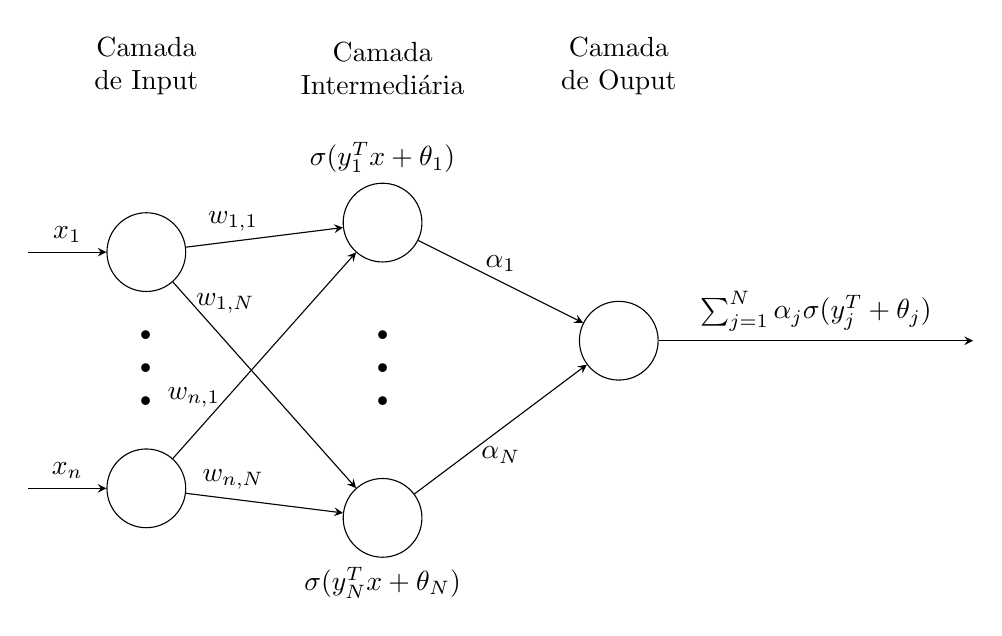
\begin{tikzpicture}[x=1.5cm, y=1.5cm, yshift=-1, >=stealth]

\foreach \m/\l [count=\y] in {1,missing,2}
  \node [every neuron/.try, neuron \m/.try] (input-\m) at (0,1.75-\y) {};

\foreach \m [count=\y] in {1,missing,2}
  \node [every neuron/.try, neuron \m/.try ] (hidden-\m) at (2,2.25-\y*1.25) {};

\foreach \m [count=\y] in {1}
  \node [every neuron/.try, neuron \m/.try ] (output-\m) at (4,1-\y) {};

\foreach \l [count=\i] in {1,n}
  \draw [<-] (input-\i) -- ++(-1,0)
    node [above, midway] {$x_\l$};

%% \foreach \l [count=\i] in {1,n}
%%   \node [above] at (hidden-\i.north) {$H_\l$};
\node [above] at (hidden-1.north) {\( \sigma (y_{ 1 }^{ T }x + \theta_{ 1 }) \)};
\node [below] at (hidden-2.south) {\( \sigma (y_{ N }^{ T }x + \theta_{ N }) \)};

\foreach \l [count=\i] in {1}
  \draw [->] (output-\i) -- ++(3,0)
    node [above, midway] {\( \sum_{ j=1 }^{ N } \alpha_{ j } \sigma (y_{ j }^{ T } + \theta_{ j }) \)};

%% \foreach \i in {1,...,2}
%%   \foreach \j in {1,...,2}
%%     \draw [->] (input-\i) -- (hidden-\j)
%%         node [above,pos=.2] {\( y_{ 1 }^{ (1) } \)};
\draw [->] (input-1) -- (hidden-1)
    node [above, pos=.3] {\( w_{ 1,1 } \)};
\draw [->] (input-2) -- (hidden-1)
    node [above, pos=.2, xshift=-2mm] {\( w_{ n,1 } \)};
\draw [->] (input-1) -- (hidden-2)
    node [above, pos=.2,xshift=2mm] {\( w_{ 1,N } \)};
\draw [->] (input-2) -- (hidden-2)
    node [above, pos=.3] {\( w_{ n,N } \)};

%% \foreach \i in {1,...,2}
%%   \foreach \j in {1}
%%     \draw [->] (hidden-\i) -- (output-\j);
\draw [->] (hidden-1) -- (output-1)
    node [above, midway] {\( \alpha_{ 1 } \)};
\draw [->] (hidden-2) -- (output-1)
    node [below, midway, yshift=-1mm] {\( \alpha_{ N } \)};

\foreach \l [count=\x from 0] in {de Input, Intermediária, de Ouput}
  \node [align=center, above] at (\x*2,2) {Camada \\ \l};

\end{tikzpicture}